\documentclass[11pt]{article}
\usepackage[margin=1in]{geometry}
\usepackage{graphicx}
\usepackage{booktabs}
\usepackage{float}
\usepackage{hyperref}
\usepackage{amsmath}
\usepackage{amssymb}
\usepackage{xcolor}
\hypersetup{colorlinks=true,linkcolor=blue,urlcolor=blue,citecolor=blue}
\setlength{\parskip}{0.55em}
\setlength{\parindent}{0pt}

\title{Federated Optimization on MIMIC-IV ICU Mortality}
\author{Federated Learning Optimization Project}
\date{\today}
\begin{document}
\maketitle

\begin{abstract}
This report extends the UCI HAR federated optimization project to MIMIC-IV ICU mortality prediction. The experiment keeps the same optimization core: FedAvg convergence, CVaR-style fairness, linear-programming communication shadow prices, and genetic hyperparameter search. The clinical task is more difficult than UCI HAR because it is binary, imbalanced, and naturally non-IID across ICU care units. The final cohort contains 73141 ICU stays, 1021 engineered features, and 9 federated ICU clients.
\end{abstract}

\tableofcontents
\newpage

\section{Problem Definition}
The goal is to predict in-hospital mortality for an ICU stay using information available in the first 24 hours after ICU admission. Each federated client is an ICU care unit identified by \texttt{first\_careunit}. This is a natural non-IID split because MICU, SICU, CVICU, Neuro ICU, and other units treat different populations with different mortality rates.

\section{Preprocessing and Cohort}
The preprocessing stage joined \texttt{icustays}, \texttt{admissions}, and \texttt{patients} to define the cohort and label. It then joined chart events, lab events, input events, output events, procedure events, prescriptions, diagnoses, procedures, services, and transfers. Time-stamped clinical event tables were restricted to the first 24 hours after ICU admission to reduce leakage. Numeric events were aggregated into per-stay mean, min, max, standard deviation, and count features where appropriate.

\begin{table}[H]
\centering
\caption{MIMIC-IV model matrix summary}
\label{tab:dataset}
\begin{tabular}{lrrrrrrrr}
\toprule
rows & features & clients & positive\_label & negative\_label & mortality\_rate & train\_rows & test\_rows & prediction\_window\_hours \\
\midrule
73141.0000 & 1021.0000 & 9.0000 & 8340.0000 & 64801.0000 & 0.1140 & 54853.0000 & 18288.0000 & 24.0000 \\
\bottomrule
\end{tabular}
\end{table}

\begin{table}[H]
\centering
\caption{Federated ICU client summary}
\label{tab:clients}
\begin{tabular}{lrrrrr}
\toprule
client\_id & client\_name & rows & mortality\_rate & deaths & alive \\
\midrule
2.0000 & Medical Intensive Care Unit (MICU) & 15940.0000 & 0.1478 & 2356.0000 & 13584.0000 \\
3.0000 & Medical/Surgical Intensive Care Unit (MICU/SICU) & 12661.0000 & 0.1456 & 1844.0000 & 10817.0000 \\
0.0000 & Cardiac Vascular Intensive Care Unit (CVICU) & 11572.0000 & 0.0425 & 492.0000 & 11080.0000 \\
7.0000 & Surgical Intensive Care Unit (SICU) & 11192.0000 & 0.1188 & 1330.0000 & 9862.0000 \\
8.0000 & Trauma SICU (TSICU) & 8668.0000 & 0.1039 & 901.0000 & 7767.0000 \\
1.0000 & Coronary Care Unit (CCU) & 8319.0000 & 0.1285 & 1069.0000 & 7250.0000 \\
4.0000 & Neuro Intermediate & 2015.0000 & 0.0199 & 40.0000 & 1975.0000 \\
6.0000 & Neuro Surgical Intensive Care Unit (Neuro SICU) & 1757.0000 & 0.1633 & 287.0000 & 1470.0000 \\
5.0000 & Neuro Stepdown & 1017.0000 & 0.0206 & 21.0000 & 996.0000 \\
\bottomrule
\end{tabular}
\end{table}

\section{EDA}
\begin{figure}[H]
\centering
\includegraphics[width=0.86\textwidth]{../outputs/full_mimic_iv/plots/eda/mortality_label_distribution.png}
\caption{Mortality label imbalance in the final cohort.}
\label{fig:label}
\end{figure}
\begin{figure}[H]
\centering

\includegraphics[width=0.86\textwidth]{../outputs/full_mimic_iv/plots/eda/client_sample_counts.png}
\caption{ICU stays per federated client.}
\label{fig:client-counts}
\end{figure}
\begin{figure}[H]
\centering
\includegraphics[width=0.86\textwidth]{../outputs/full_mimic_iv/plots/eda/client_mortality_rates.png}
\caption{Mortality rate differs strongly by ICU care unit.}
\label{fig:client-mortality}
\end{figure}
\begin{figure}[H]
\centering
\includegraphics[width=0.86\textwidth]{../outputs/full_mimic_iv/plots/eda/client_noniid_js_divergence.png}
\caption{Non-IID label severity measured by Jensen-Shannon divergence.}
\label{fig:noniid}
\end{figure}
\begin{figure}[H]
\centering
\includegraphics[width=0.86\textwidth]{../outputs/full_mimic_iv/plots/eda/pca_by_mortality.png}
\caption{Two-dimensional PCA visualization by mortality label. PCA is used for EDA only, not as the main training representation.}
\label{fig:pca-mortality}
\end{figure}
\begin{figure}[H]
\centering

\includegraphics[width=0.86\textwidth]{../outputs/full_mimic_iv/plots/eda/pca_3d_by_client.png}
\caption{Three-dimensional PCA visualization by ICU client.}
\label{fig:pca-client-3d}
\end{figure}

\section{Training Configuration}
All main validation uses ten seeds: \texttt{7,11,19,23,29,31,37,41,43,47}. The MIMIC model is a tabular MLP with 796 inputs and two output classes. Weighted cross entropy is used because mortality prevalence is about 11.4 percent. Early stopping uses loss with \texttt{max\_rounds=1000}, \texttt{patience=25}, and \texttt{min\_delta=0.0005}.

\section{Main Results}
The strongest mean AUPRC in this run is \texttt{fedavg\_default} with mean AUPRC 0.6316. Accuracy is reported, but clinical interpretation focuses more on AUPRC, sensitivity, specificity, balanced accuracy, and worst-client metrics.

\begin{table}[H]
\centering
\caption{Method comparison across seeds}
\label{tab:methods}
\begin{tabular}{lrrrrrrrrrr}
\toprule
method & n & final\_accuracy\_mean & final\_auroc\_mean & final\_auprc\_mean & final\_balanced\_accuracy\_mean & final\_sensitivity\_mean & final\_specificity\_mean & final\_worst\_client\_recall\_mean & total\_comm\_until\_stop\_mean & stopped\_round\_mean \\
\midrule
fedavg\_default & 10.0000 & 0.8776 & 0.8889 & 0.6316 & 0.7942 & 0.7164 & 0.8721 & 0.2100 & 571901632.0000 & 47.2000 \\
cvar\_0 & 10.0000 & 0.8640 & 0.8860 & 0.6260 & 0.7875 & 0.7043 & 0.8707 & 0.2600 & 645812648.0000 & 53.3000 \\
cvar\_0.5 & 10.0000 & 0.8732 & 0.8758 & 0.6137 & 0.7796 & 0.6916 & 0.8676 & 0.1600 & 712453728.0000 & 58.8000 \\
cvar\_0.75 & 10.0000 & 0.8663 & 0.8783 & 0.6146 & 0.7846 & 0.7146 & 0.8546 & 0.2400 & 579171568.0000 & 47.8000 \\
cvar\_0.9 & 10.0000 & 0.8663 & 0.8783 & 0.6146 & 0.7846 & 0.7146 & 0.8546 & 0.2400 & 579171568.0000 & 47.8000 \\
cvar\_0.95 & 10.0000 & 0.8663 & 0.8783 & 0.6146 & 0.7846 & 0.7146 & 0.8546 & 0.2400 & 579171568.0000 & 47.8000 \\
centralized & 10.0000 & 0.9078 & 0.8782 & 0.5851 & 0.7598 & 0.5890 & 0.9306 & 0.1600 & 0.0000 & 31.8000 \\
local\_only & 1.0000 & 0.9036 & 0.8690 & 0.4591 & 0.7144 & 0.4895 & 0.9392 & 0.0000 & 0.0000 & 50.0000 \\
grid\_best\_validated & 10.0000 & 0.9013 & 0.8595 & 0.5981 & 0.7719 & 0.6299 & 0.9138 & 0.1300 & 359134838.4000 & 49.4000 \\
ga\_best\_validated & 10.0000 & 0.8670 & 0.8839 & 0.6290 & 0.7876 & 0.7213 & 0.8539 & 0.2500 & 318423196.8000 & 43.8000 \\
\bottomrule
\end{tabular}
\end{table}

\begin{table}[H]
\centering
\caption{Final selected model clinical metrics}
\label{tab:clinical}
\begin{tabular}{lrrrrrrrrr}
\toprule
accuracy & balanced\_accuracy & auroc & auprc & sensitivity & specificity & precision\_ppv & npv & f1\_death & brier \\
\midrule
0.8403 & 0.8156 & 0.9055 & 0.6531 & 0.7837 & 0.8476 & 0.3981 & 0.9682 & 0.5280 & 0.1131 \\
\bottomrule
\end{tabular}
\end{table}

\section{Training Dynamics}
\begin{figure}[H]
\centering
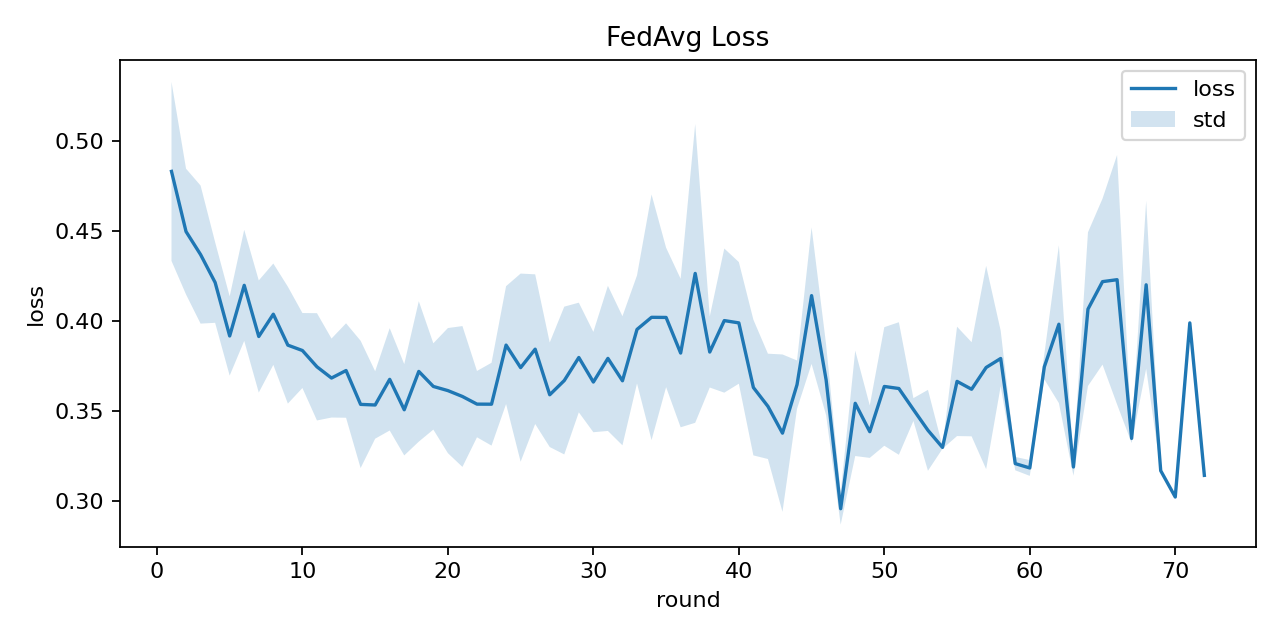
\includegraphics[width=0.86\textwidth]{../outputs/full_mimic_iv_training/plots/training/loss_vs_rounds.png}
\caption{FedAvg loss across communication rounds.}
\label{fig:loss}
\end{figure}
\begin{figure}[H]
\centering
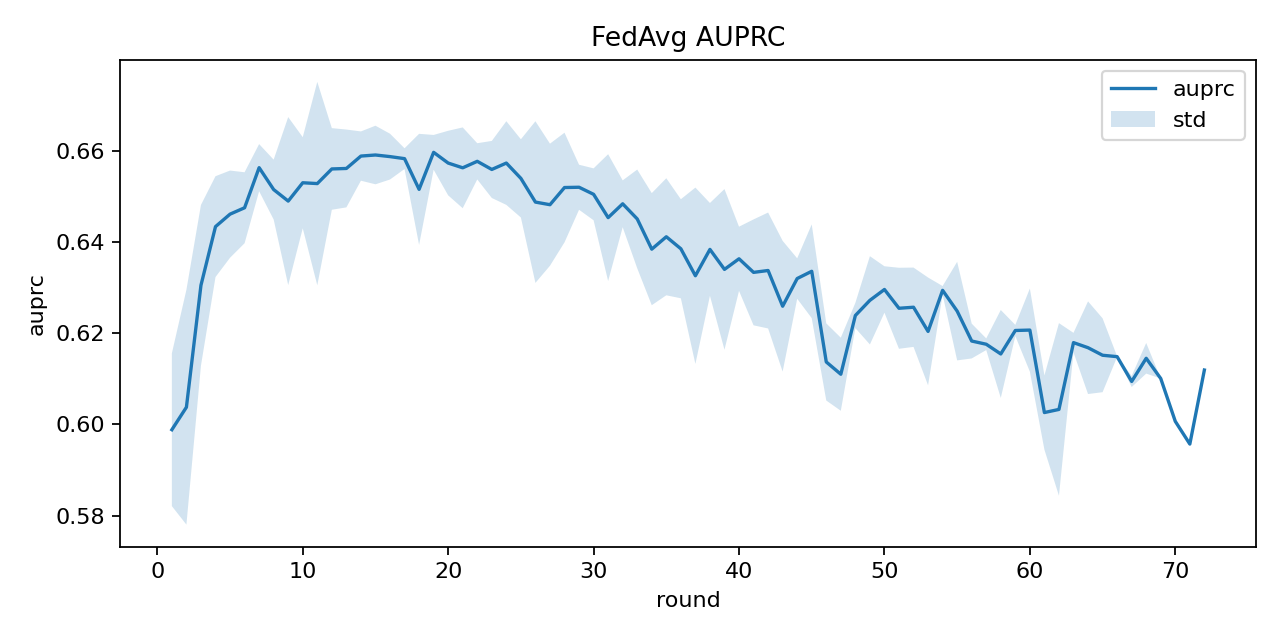
\includegraphics[width=0.86\textwidth]{../outputs/full_mimic_iv_training/plots/training/auprc_vs_rounds.png}
\caption{AUPRC across communication rounds.}
\label{fig:auprc-rounds}
\end{figure}
\begin{figure}[H]
\centering
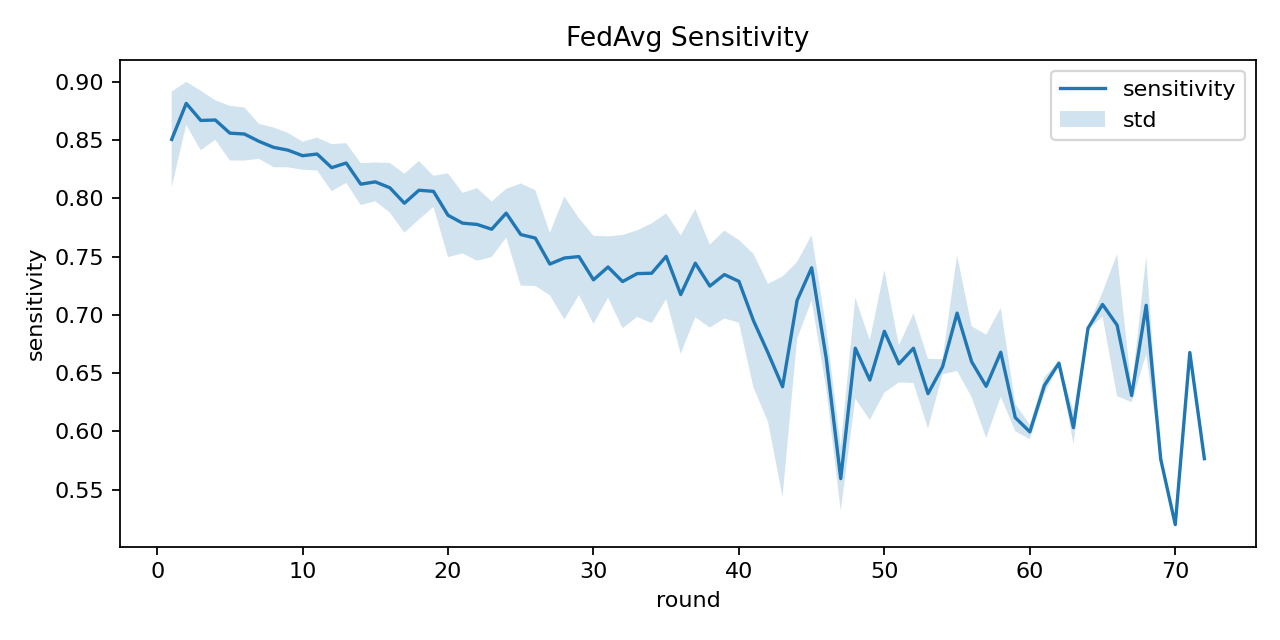
\includegraphics[width=0.86\textwidth]{../outputs/full_mimic_iv_training/plots/training/sensitivity_vs_rounds.png}
\caption{Mortality sensitivity across communication rounds.}
\label{fig:sens-rounds}
\end{figure}
\begin{figure}[H]
\centering
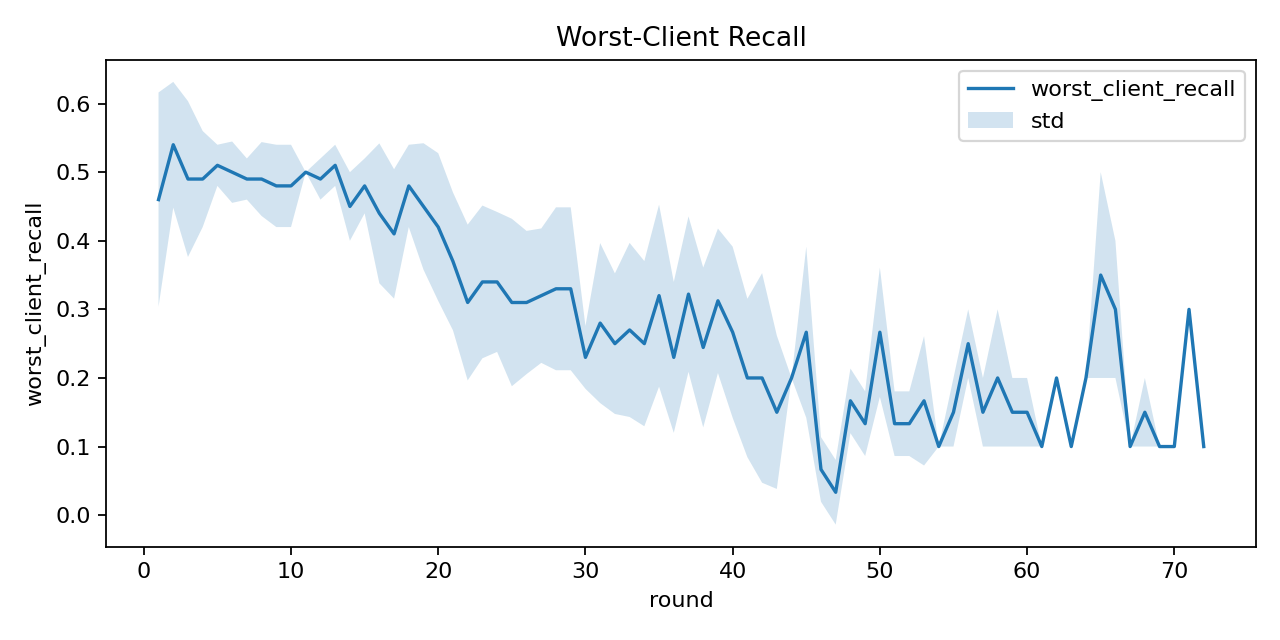
\includegraphics[width=0.86\textwidth]{../outputs/full_mimic_iv_training/plots/training/worst_client_recall_vs_rounds.png}
\caption{Worst-client mortality recall across rounds.}
\label{fig:worst-recall}
\end{figure}

\section{Fairness and Client-Level Analysis}
\begin{figure}[H]
\centering
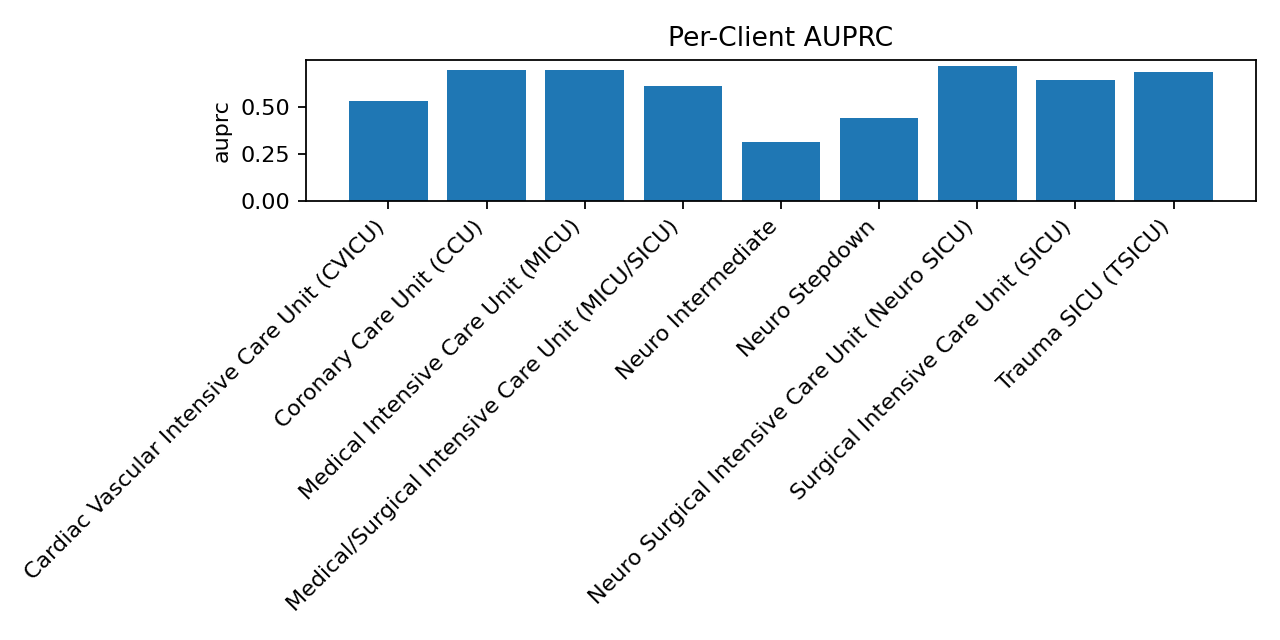
\includegraphics[width=0.86\textwidth]{../outputs/full_mimic_iv_training/plots/fairness/per_client_auprc.png}
\caption{Per-client AUPRC for the final selected model.}
\label{fig:client-auprc}
\end{figure}
\begin{figure}[H]
\centering
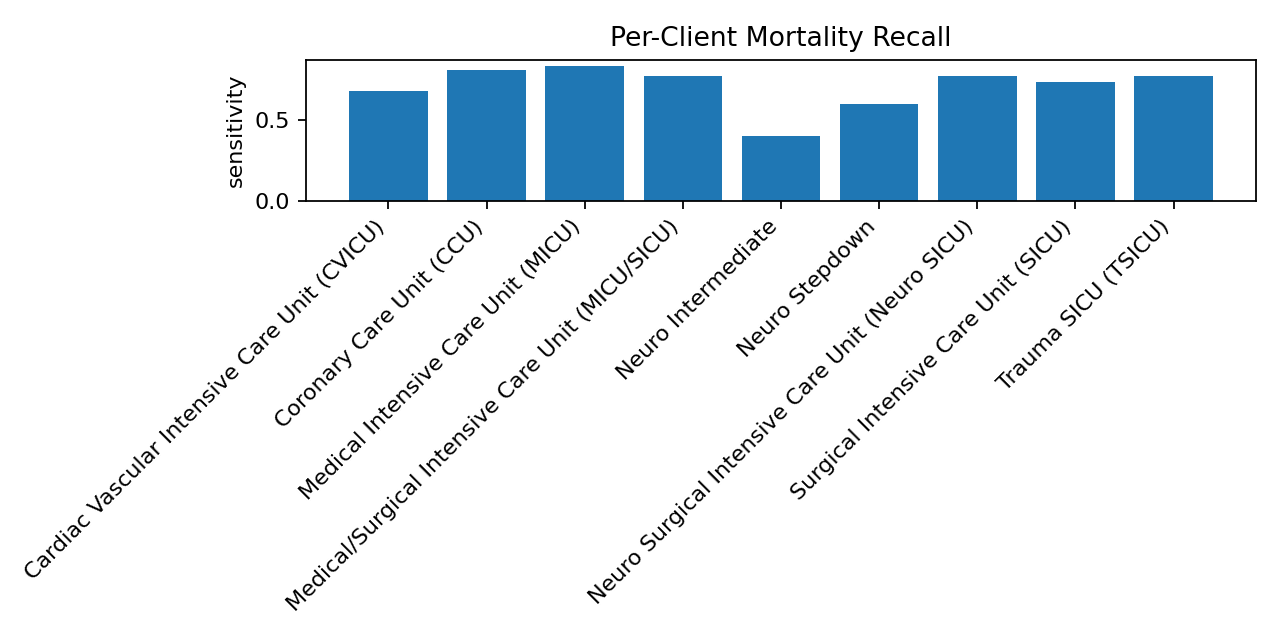
\includegraphics[width=0.86\textwidth]{../outputs/full_mimic_iv_training/plots/fairness/per_client_mortality_recall.png}
\caption{Per-client mortality recall for the final selected model.}
\label{fig:client-recall}
\end{figure}
\begin{figure}[H]
\centering
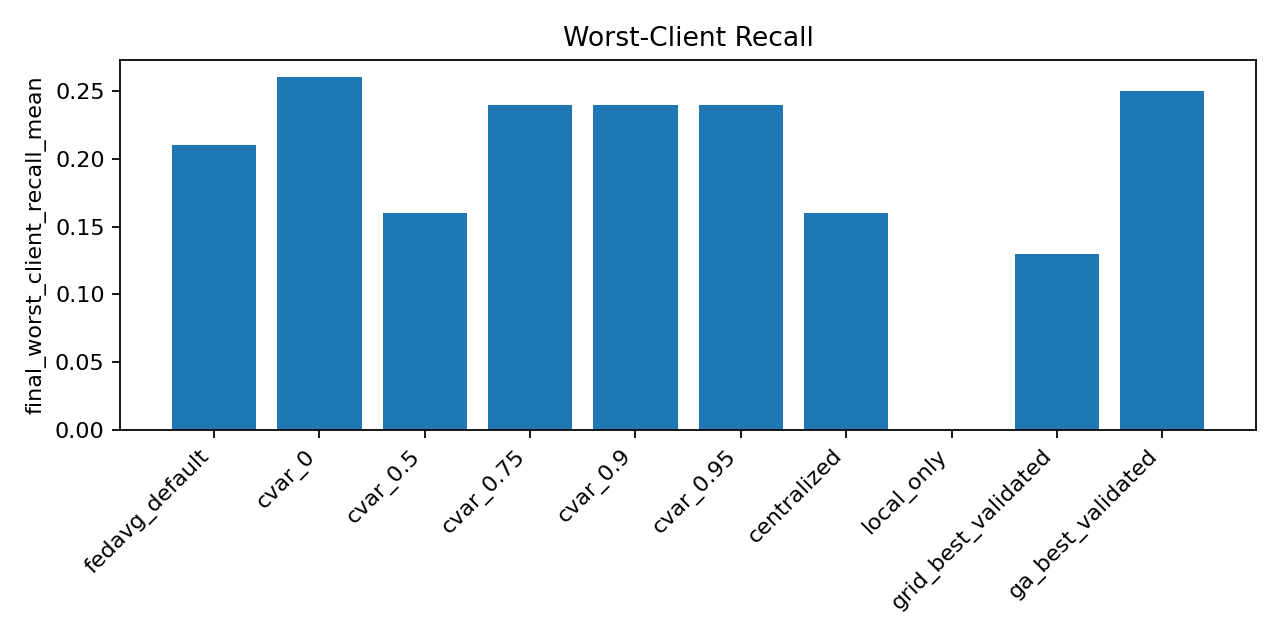
\includegraphics[width=0.86\textwidth]{../outputs/full_mimic_iv_training/plots/fairness/worst_client_recall_by_method.png}
\caption{Worst-client recall by method.}
\label{fig:worst-method}
\end{figure}

\section{Clinical Classification}
\begin{figure}[H]
\centering
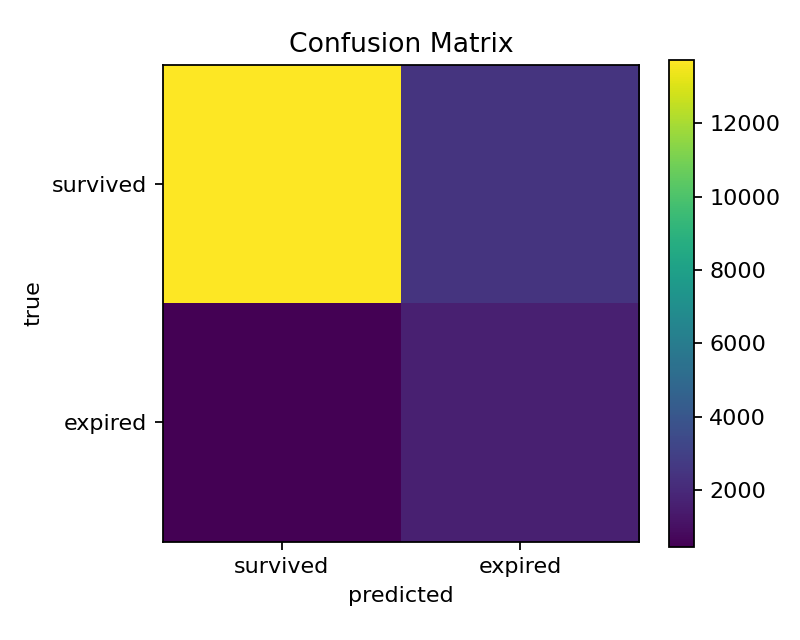
\includegraphics[width=0.86\textwidth]{../outputs/full_mimic_iv_training/plots/classification/confusion_matrix.png}
\caption{Confusion matrix for the final selected model.}
\label{fig:cm}
\end{figure}
\begin{figure}[H]
\centering
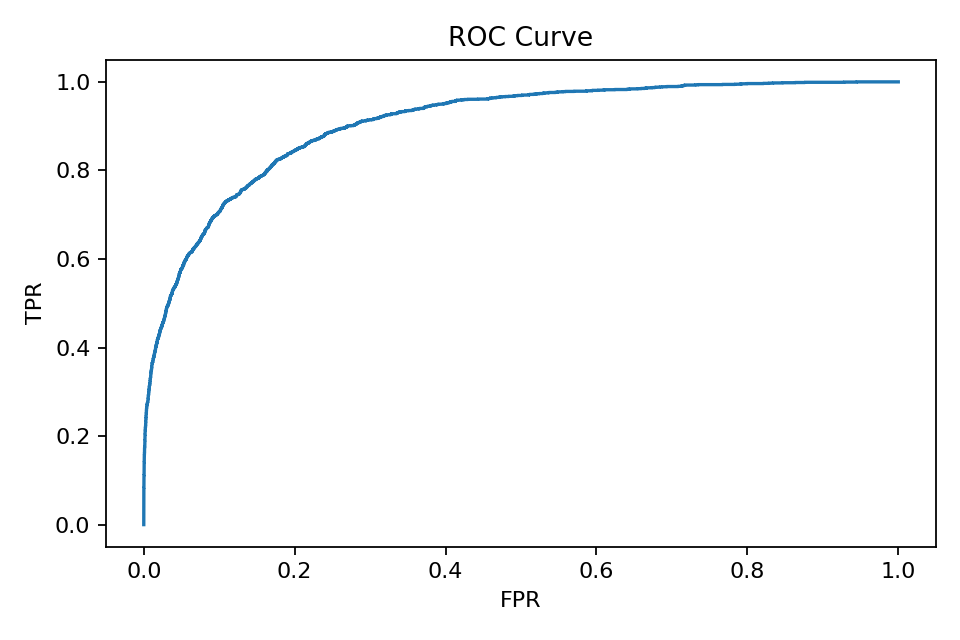
\includegraphics[width=0.86\textwidth]{../outputs/full_mimic_iv_training/plots/classification/roc_curve.png}
\caption{ROC curve.}
\label{fig:roc}
\end{figure}
\begin{figure}[H]
\centering
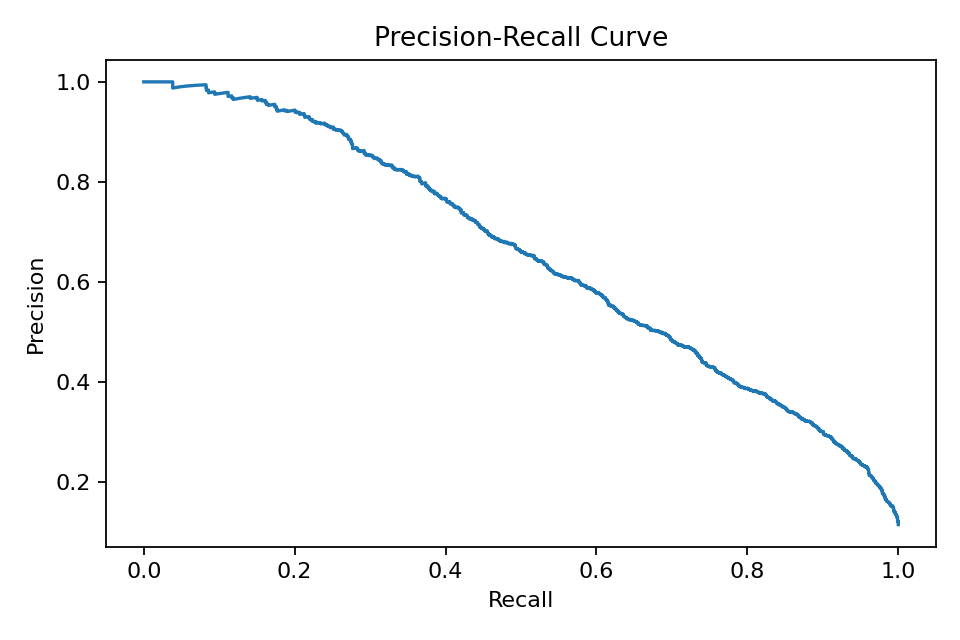
\includegraphics[width=0.86\textwidth]{../outputs/full_mimic_iv_training/plots/classification/precision_recall_curve.png}
\caption{Precision-recall curve, which is especially important for imbalanced mortality prediction.}
\label{fig:pr}
\end{figure}

\section{Search and Communication Optimization}
The genetic search evaluated 48 candidate configurations. The best raw vector was \texttt{[1.2660918762649054, 3.4847698845669535, 0.005769185832593745]}. Grid and GA candidates were then validated with the same ten-seed protocol as FedAvg and CVaR.

\begin{figure}[H]
\centering
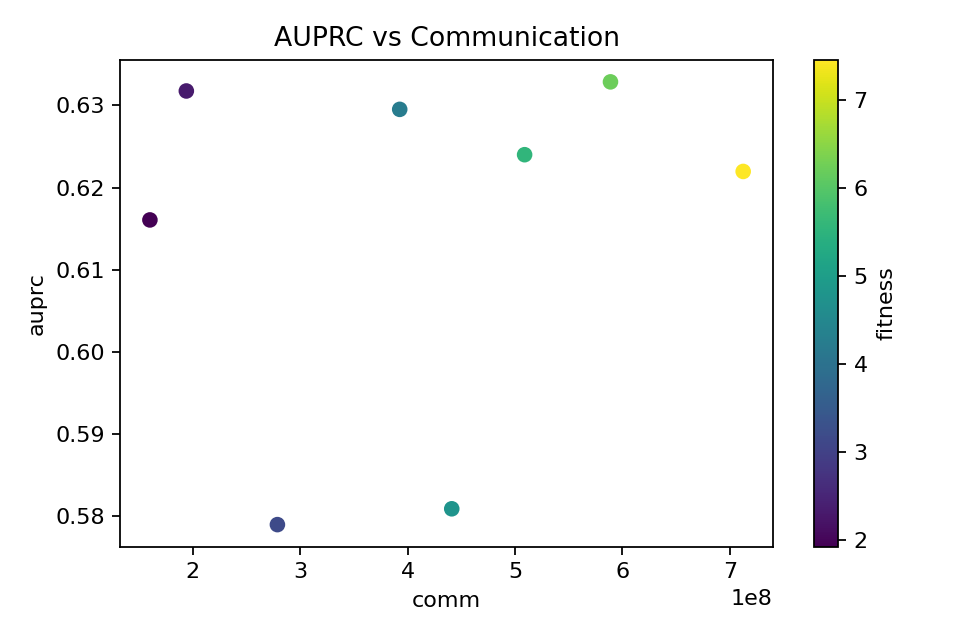
\includegraphics[width=0.86\textwidth]{../outputs/full_mimic_iv_training/plots/search/auprc_vs_communication_scatter.png}
\caption{Search candidates plotted by AUPRC and communication.}
\label{fig:search-scatter}
\end{figure}
\begin{figure}[H]
\centering
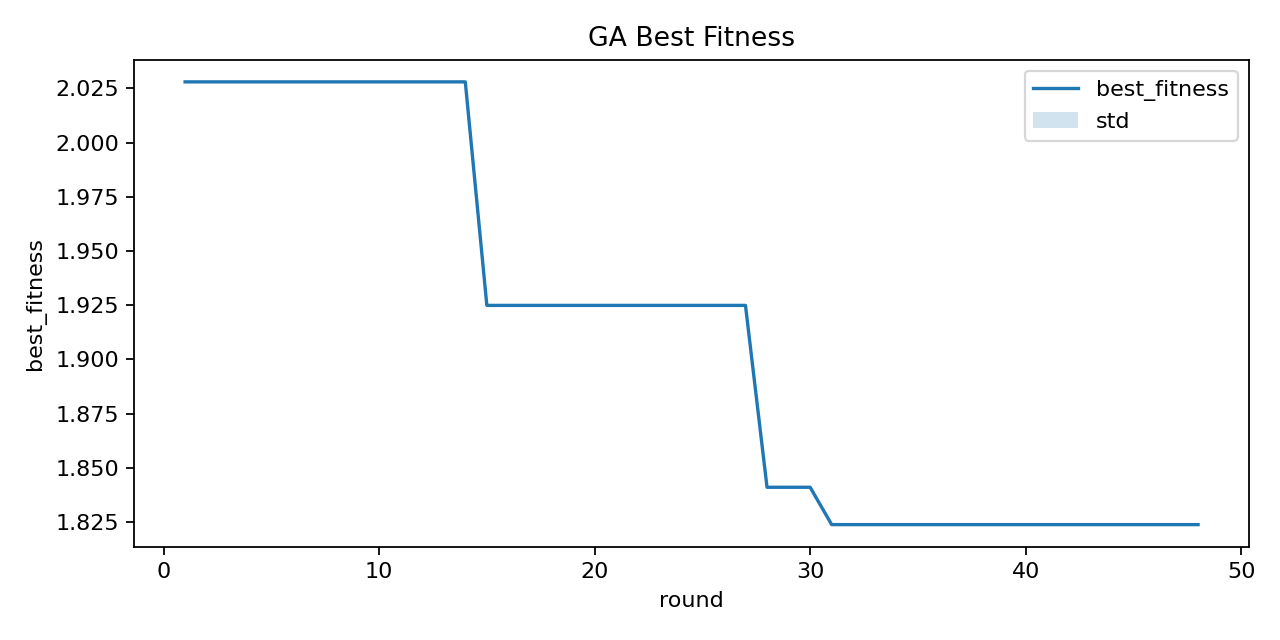
\includegraphics[width=0.86\textwidth]{../outputs/full_mimic_iv_training/plots/search/ga_fitness_vs_evaluations.png}
\caption{Best genetic-search fitness over evaluations.}
\label{fig:ga}
\end{figure}
\begin{figure}[H]
\centering
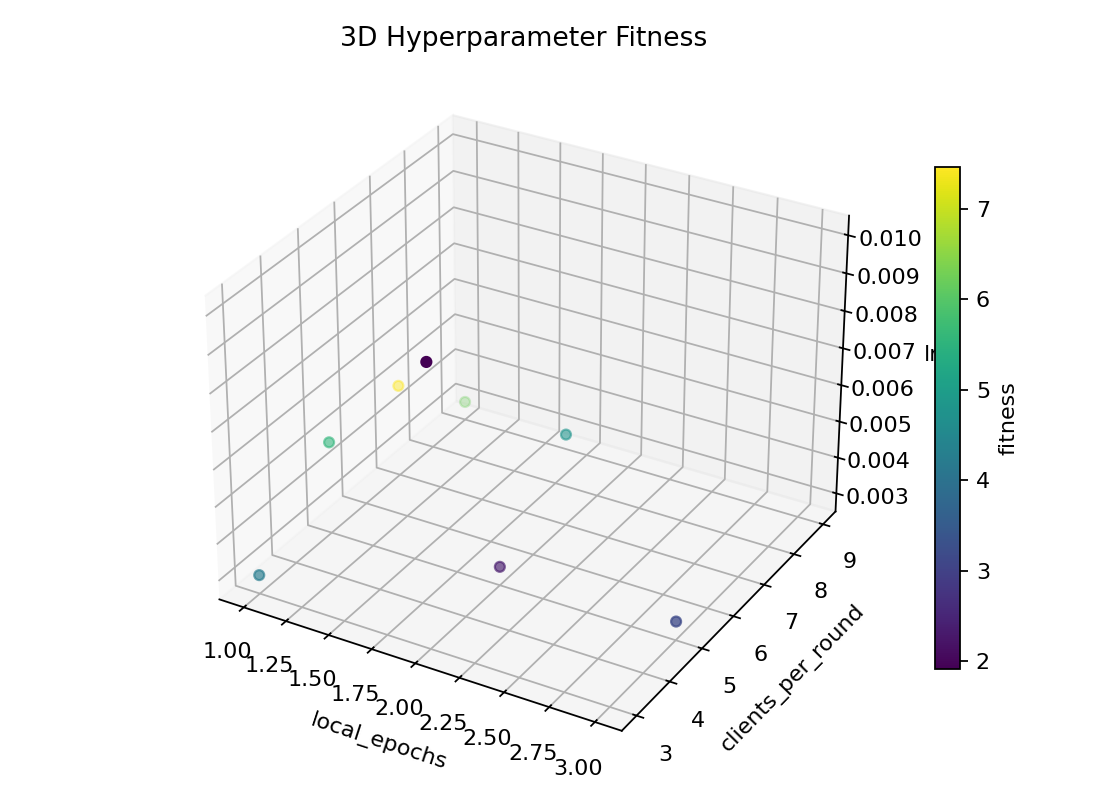
\includegraphics[width=0.86\textwidth]{../outputs/full_mimic_iv_training/plots/search/hyperparameter_3d_fitness.png}
\caption{Three-dimensional hyperparameter search landscape.}
\label{fig:hp3d}
\end{figure}
\begin{figure}[H]
\centering
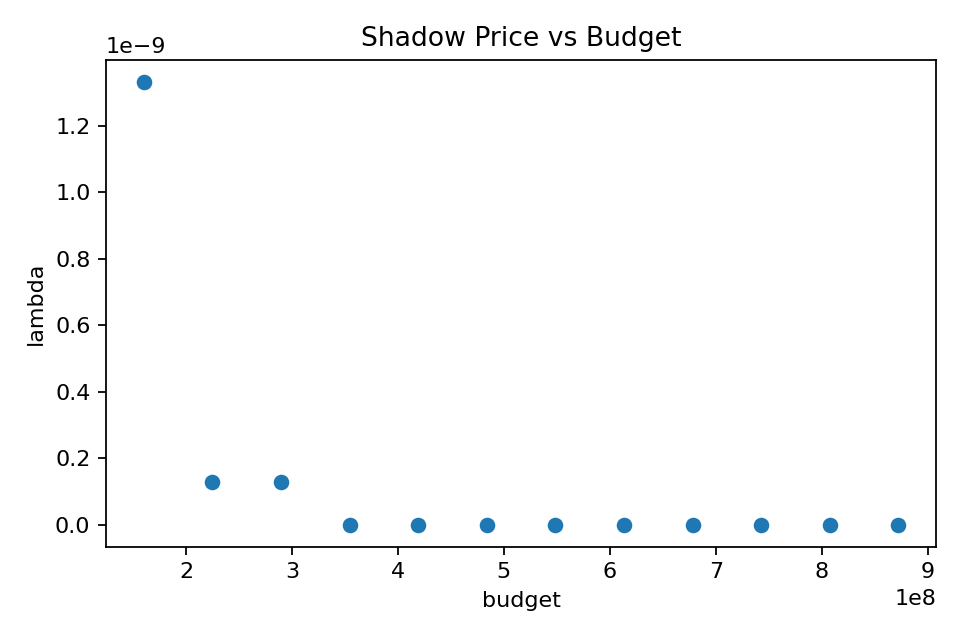
\includegraphics[width=0.86\textwidth]{../outputs/full_mimic_iv_training/plots/optimization/shadow_price_vs_budget.png}
\caption{LP communication shadow price by budget.}
\label{fig:lambda}
\end{figure}
\begin{figure}[H]
\centering
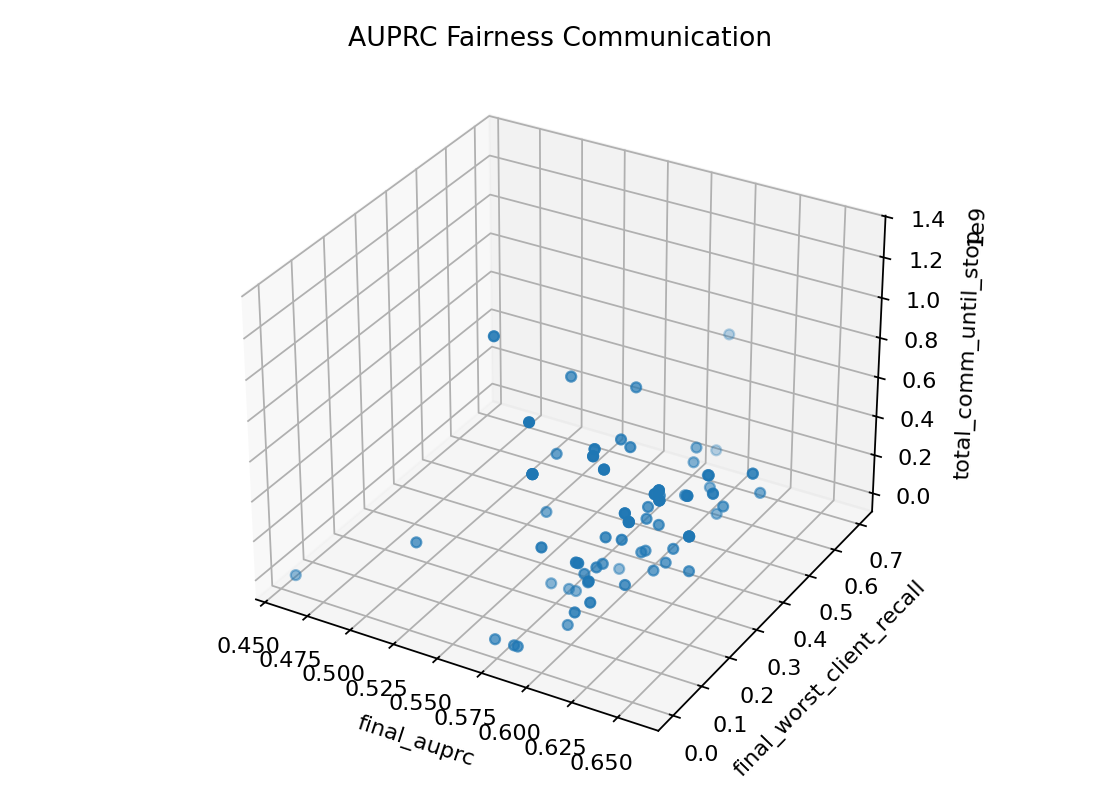
\includegraphics[width=0.86\textwidth]{../outputs/full_mimic_iv_training/plots/optimization/auprc_fairness_communication_3d.png}
\caption{Three-way tradeoff between AUPRC, fairness, and communication.}
\label{fig:tradeoff3d}
\end{figure}

\section{Runtime}
\begin{table}[H]
\centering
\caption{Runtime by pipeline stage}
\label{tab:runtime}
\begin{tabular}{lr}
\toprule
stage & seconds \\
\midrule
load\_mimic\_arrays & 0.2641 \\
fedavg\_default & 185.3920 \\
cvar\_sweep & 989.0590 \\
baselines & 222.3467 \\
search & 1256.8964 \\
predictions\_metrics & 9.6077 \\
lp\_diagnostics & 0.1571 \\
diagnostics & 1.2190 \\
plots & 0.9817 \\
artifacts & 0.0200 \\
\bottomrule
\end{tabular}
\end{table}

\section{Limitations}
This run is a strong federated optimization baseline, but it should be interpreted carefully. Some administrative features may reflect coding processes rather than pure early physiology, so leakage-sensitive ablations should be used in future work. The local-only baseline is not directly comparable to ten-seed global methods because it trains separate client models. Finally, high AUROC does not guarantee high death recall in every ICU unit, so false-negative analysis remains central.

\section{Artifacts}
The main output folder is \texttt{outputs/full\_mimic\_iv\_training}. It contains raw round logs, method summaries, clinical metrics, predictions, calibration outputs, LP diagnostics, search history, plots, model checkpoints, and report drafts. The preprocessing folder \texttt{outputs/full\_mimic\_iv} contains the joined model matrix, EDA outputs, and the saved preprocessor.

\end{document}
